\documentclass[11pt]{article} %Sets the default text size to 11pt and class to article.
\usepackage{graphicx}
\usepackage{amsmath}
\newcommand{\BigO}[1]{\ensuremath{\operatorname{O}\bigl(#1\bigr)}}
%------------------------Dimensions--------------------------------------------
\topmargin=-.5in %length of margin at the top of the page (1 inch added by default)
\oddsidemargin=-0.2in %length of margin on sides for odd pages
\evensidemargin=0in %length of margin on sides for even pages
\textwidth=6.5in %How wide you want your text to be
\marginparwidth=0.5in
\headheight=0pt %1in margins at top and bottom (1 inch is added to this value by default)
\headsep=0pt %Increase to increase white space in between headers and the top of the page
\textheight=10.0in %How tall the text body is allowed to be on each page
\pagestyle{empty}
\begin{document}
\centerline{{ \LARGE \bf Problem Set 7}} 
\centerline{CSCI 3104 Spring 2014} 
\centerline{Cristobal Salazar}
\centerline{07/22}
\centerline{Partner: Alex Tsankov}

\noindent{\Large \bf Problem 1}
\\
\\
\indent{\large a) An edge list takes $O(E)$ time in a worst case scenario, because it has to check each of the edges for a possible connection between two vertices.}
\\

\indent{\large b) An adjacency list representation takes $O(V)$ time to determine edges between two different vertices. This because, in a worst case scenario, it has to scan through all of the vertices to discover possible connections. }
\\

\indent{\large c) An adjacency matrix representation takes $O(1)$ time to determine connections between two different vertices because all it has to do is access an element in an array matrix.}
\\
\\
\noindent{\Large \bf Problem 2}
\\
\\
\indent{\large The algorithm that can work for this conversion would involve two parts: Making sure that the edges between two vertices are the same on both ends (ex. a $\to$ b, b $\to$ a), and then removing duplicates from each of the edge lists (ex. a $\to$ b,a $\to$ c, a $\to$ e). The first part will take $O(V)$ time, and the second part will take $O(E)$ time, leading to a combined performance of $O(V+E)$ }
\\
\\
\indent{\large Our first step requires us to remove duplicates from each of the adjacency lists. Because there is a limited number of possible chars, our algorithm will take $O(n)$ time for each list, essentially checking the node for duplicate connections, for a total of $O(V)$ time for the total set .}
\\
\\
\indent{\large Our second step requires us to select a linked list to work on, in our case we can do edge set A representing the connections between "a" and the other nodes ("b", "c", "d", "e"). With edge set A selected, we then scan through all of the other edge sets, not already included in edge set A [ex: if A begins with edges to (c,b), we only check edge sets that are not included and not itself, in this case: (d,e)] looking for connections to "a". If we find an edge to "a", for example in "d" we add it to the linked list, if it isn't we just continue until we reach the end of possible vertices and begin with the next edge set. We then go through the rest of the edge sets, in our case, continuing with edge set "b" and checking if we have any connections to other lists, adding connections as we go. } 
\\
\\
\noindent{\Large \bf Problem 3}
\\

\indent{\large a) To prove this using contradiction, we will assume that tree $T = (V,E)$ is not a bipartite graph. By definition, this means no partition exists on $V$ into subsets $R$ and $L$ where every edge $(u,v)\in E$ has $u \in R$ AND $v \in L$. This implies that for every partition of vertices, there exists at least one edge where both $u,v \in R$ or $u,v \in L$. To make this partition possible, then there must be a loop in the tree. If a tree has a loop of any kind, then by definition it is no longer a tree. Therefore we can conclude that to make a tree non-bipartite we must have an edge between two vertices that creates a loop in the tree(making it not a tree), this implies that all trees must be bipartite.}
\\

\indent{\large b) To check to see if a graph is bipartite, we can use an adapted version of Breadth First Search(BFS). We will start by making all vertices white. Then we will make the source vertex red. Then we will make the first breadth black, then next breadth red, the next black, and so on as we traverse the graph. If at any point two red nodes or two black nodes are connected to each other, then we will know the graph is NOT bipartite. This algorithm will have a running time of $O(V+E)$. Making all of the nodes white will take $\Theta(V)$, and the traversal will take $O(E)$. Psuedo-Code:}
\begin{verbatim}
isBipartite(G, s){ \\takes input graph, and source node
  for i=0 to n {v[i] = WHITE; p[i] = NULL; d[i] = INF} \\sets all nodes to white
  Q = new Queue
  v[s] = RED \\sets source to red
  d[s] = 0 \\distance to source of first node is 0
  enqueue(Q, s) \\puts s in queue
  color = 0 \\Red is even level, black is odd level 
  while(Q.length >= 0){
    x = dequeue(Q) \\dequeue first the current node 
    for(each neighbor y of x){
      if(v[y] == WHITE){ 
        if(color % 2 == 0)
          v[y] = RED
        else
          v[y] = BLACK
      }
      if(v[y] == v[x]) \\checking if the colors of neighbours are the same. 
        return false
    }
  }
  return true
}
\end{verbatim}

\noindent{\Large \bf Problem 4}
\\
\indent{\large  For Snape's algorithm we must first notice that if $a_{ij}=1$, then $(i,j)\in E$ and vertex $i$ cannot be the universal sink because there is an outgoing edge. Therefore if row $i$ contains 1, then vertex $i$ is not a universal sink. We also know, that if $a_{ij}$ AND $i\neq j$, then $(i,j) \notin E$ and vertex $j$ cannot be in a universal sink. Therefore, if column $j$ contains $0$ in every position(except the diagonal entry $(i,j)$), then $j$ cannot be the universal sink. With these observations being true, we know that if we keep adding up the number of times $a_{ij} == 1$, and if we exceed the bounds of the adjacency matrix, then it is not a universal sink. Like so: }
\begin{verbatim}
isSink(G){ \\takes input adjacency matrix 
  x = 1 \\this is to represent rows
  y = 1 \\ this is to represent columns 
  while(x <= |G.rows()| && y <= |G|.columns()){ \\while in bounds of the matrix.  
    if(G[x,y] == 1) \\checks current adjacency in matrix, increment in x 
      x++
    else
      y++
  }
  if(x > G.rows()) \\this compares x axis to length of G rows. 
    return false
  else
    return true
}
\end{verbatim}
\newpage
\noindent{\Large \bf Problem 5}
\\

\noindent{\large Our algorithm determines the diameter by doing the following steps:\\\\1) Create a list of all vertices, we will use this to feed into our BFS algorithm, also set a diameter of 0.\\2)Run a BFS between one vertex and all other vertices not including itself.\\3) For every path between a vertex (a run of BFS), calculate the number of edges it takes to get there. This is a possible diameter. If this number is bigger than our previously set diameter, this is our new diameter. If it isn't, drop this number to save memory.\\4)Keep running steps 2 and 3 on the other nodes to find the biggest diameter of all paths.\\5)Return the final diameter when we are done going through all of the nodes, this is the longest shortest path in terms of edges it takes to traverse.}
\\
\\
\noindent{\large This algorithm satisfies the space requirement because it checks the diameter one path at a time, and if it doesn't match it throws away the path. All it needs to do is keep a diameter variable to compare the paths to and change according to size. The run time complexity for this algorithm is $O(V^2 * E)$ because it does two for loops through the vertices $O(V^2)$ and then runs BFS on them, which is $O(E)$, leading to a final run-time of $O(V^2 * E)$ }
\\

\noindent{\Large \bf Problem 6}


\noindent{\large a) To calculate the average diameter of an Erdos-Renyi random graph with a constant C = 5 we simply had to re-purpose our algorithm from the previous question.\\\\The first step is to calculate our Erdos-Renyi graphs, by using the functions given to us in the HW, we calculate the probability for each unique graph, and construct it based on the number of nodes.With our graph in place, we use our re-purposed diameter algorithm to log the diameter of each unique graph. This will become a data point for our final answer.\\\\With the ability to calculate the diameter for a series of random Erdos-Renyi graph, we need to run our code enough times to calculate an average and plot it on the graph. For each node, we construct a hundred graphs and find the diameter of each of these graphs. We then take the average of the hundred diameters to be plotted. Each dot on the graph represents the average diameter for 100 random Erdos-Renyi graphs constructed with that many nodes. When we do this we notice that our expected diameter is $O($lg n). See {\bf Fig. 1} below. }
\\
\\
\noindent{\large b) To calculate the run-time of our algorithm, we did the same process as above, except we timed and averaged how long it took to calculate the diameter of the Erdos-Renyi graph based on number of nodes. We took a total of a hundred time differences for each node number and averaged it together. We were unsure of what to predict, so we assumed going into the test a runtime of $O(V^2 + E^2)$. See {\bf Fig. 2} below for actual run time results.\\\\ The memory footprint was more difficult. We needed to find a piece of software that would be able to log memory changes in our program as time progressed. We eventually found the tool to do this, and the results can be seen below at {\bf Fig. 3}. What this tool did, was check the memory usage of our main graph aggregator that we used above at 1 second intervals, and logged the change in memory usage. In the graph below the, green "G" line is the most important one because that is the actual memory usage to store the graphs. The other lines have to do with program overhead. An important caveat is that the graph is actually much more exponential than it looks. Because of the way that the memory tracker examined the memory (in 1 second intervals), some more expensive calculations that took more than 1 second were given similar memory usages to ones that took much less than second. This leads to a logarithmic shortening of the y-axis that should be kept in mind. 
\\
\begin{figure}[ht!]
\centering
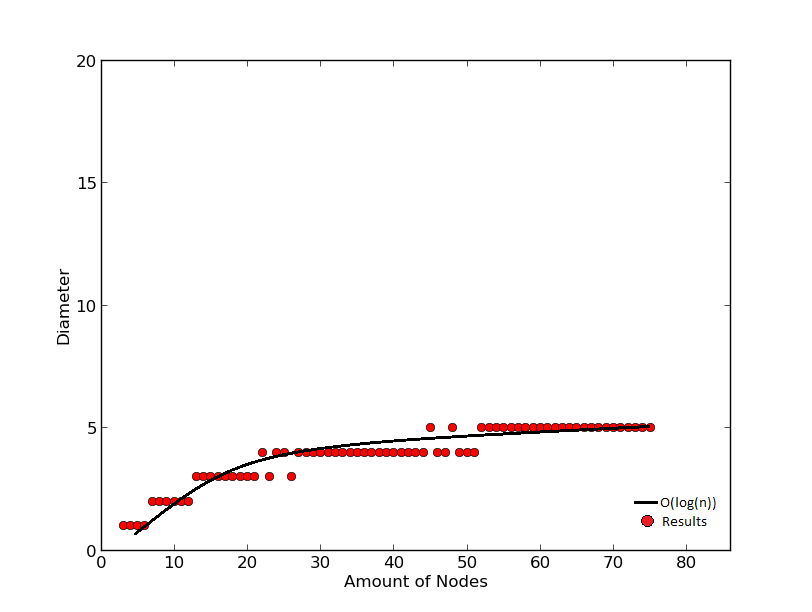
\includegraphics[width=120mm]{problem_6_a_new.png}
\caption{Average Expected Diameter of Erdos-Renyi Graphs by number of nodes.}
\label{overflow}
\end{figure}
\\
\begin{figure}[ht!]
\centering
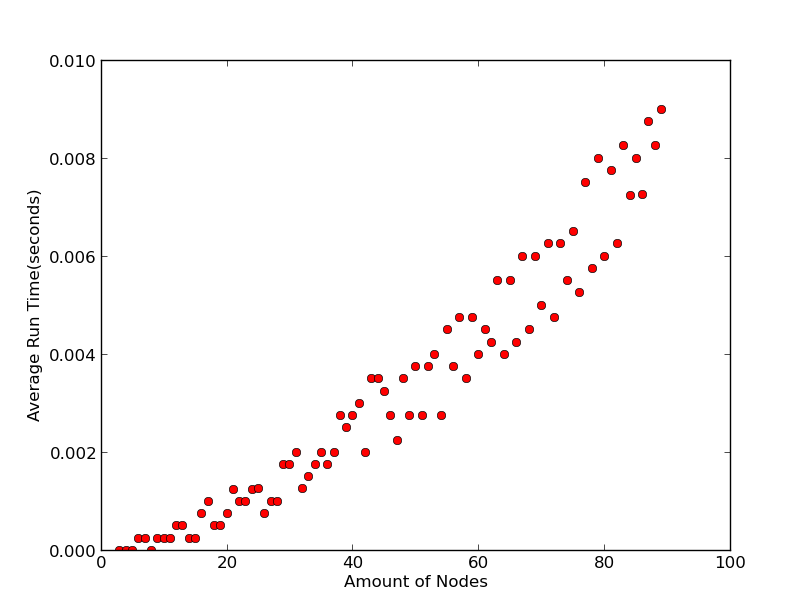
\includegraphics[width=120mm]{problem_6_b_run.png}
\caption{Average Run-Time of Erdos-Renyi Graphs by number of nodes.}
\label{overflow}
\end{figure}
\\
\\
\begin{figure}[ht!]
\centering
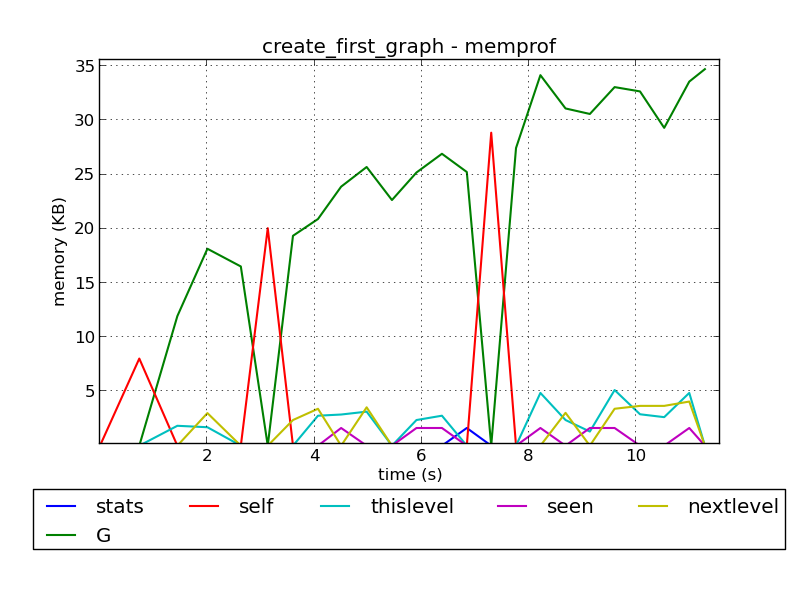
\includegraphics[width=120mm]{create_first_graph.png}
\caption{Memory usage over time, view Y-axis as logarithmic to make up for memory checker deficiencies. Memory usage is exponential.}
\label{overflow}
\end{figure}
\\
\\
\\
\\
\noindent{\Large \bf Problem 7}
\\

\indent{\large  To see that $E_{\pi}$ cannot be a breadth first tree we can run a Breadth-First Search algorithm to the following directed adjacency list: }
\begin{verbatim}
Adj[]= 
s| [a, b]                   -> a --> c
a| [c, d]                  /    \ /
b| [d, c]    visuallly:   s      \ 
c| []                      \    / \
d| []                       -> b --> d
\end{verbatim}
\indent{\large We see that in $Adj[s]$, $u$ listed before $v$. If we were running a BFS algorithm, we would add the edges $(s,u)$ and $(s, v)$ to the tree. Therefore we know $u$ will be queued before $v$. The algorithm then adds the edges $(u, w)$ and $(u, x)$ (In $Adj[u]$, the order of $w$ and $x$ are irrelevant). The mirror will also be true. So, if $Adj[s]$ lists $v$ before $u$, then our algorithm adds the edges $(s, v)$ and $(s,u)$ to the tree, where $v$ is queued before $u$, and our algorithm adds the edges $(v, w)$ and $(v, x)$ (In $Adj[v]$ the order is, again, irrelevant). Given this, we see that our algorithm will never put both edges $(u, w)$ and $(v, x)$ into the tree. Similarly, the algorithm will also never put both edges $(u, x)$ and $(v, w)$ into the tree. Therefore, $E_{\pi}$ cannot be produced by running a breadth-first search on G, no matter how the vertices
are ordered in each adjacency list.
}
\\
\\
\noindent{\Large \bf Sources}
\\
\indent $\bullet$ http://www.geeksforgeeks.org/bipartite-graph/
%this is for 3a
\\
\indent $\bullet$ http://www.geeksforgeeks.org/graph-and-its-representations/
%this is for 1a
\\
\indent $\bullet$ http://eddmann.com/posts/depth-first-search-and-breadth-first-search-in-python/
%this is for 5, the BFS algorithm reference 
\\
\indent $\bullet$ https://people.hofstra.edu/geotrans/eng/methods/diameter1.html
%this is for 5, what exactly diameter means 
\\

\noindent{\Large \bf Source Code:}


\end{document}